\documentclass[10pt,aspectratio=169]{beamer}

\usetheme[progressbar=foot]{metropolis}
\AtBeginSection{}

\usepackage{appendixnumberbeamer}
\usepackage{booktabs}
\usepackage[scale=2]{ccicons}
\usepackage{tabularx}
\usepackage{tikz}
\usetikzlibrary{arrows.meta,positioning,shapes.geometric,fit,calc}
\usepackage{xspace}
\newcommand{\themename}{\textbf{\textsc{metropolis}}\xspace}
\usepackage{comment}
\usepackage{caption}
\usepackage[
  backend=biber,
  style=authoryear
]{biblatex}

\setbeamertemplate{bibliography item}{}
\addbibresource{bibliography.bib}

\usepackage{graphicx}
\usepackage{siunitx}



%................................................................................
% COLORS

\definecolor{ukudlaBlue}{RGB}{41, 60, 135}
\definecolor{ukudlaLightBlue}{RGB}{212, 216, 231}
\definecolor{ukudlaRed}{RGB}{164, 28, 34}
\definecolor{ukudlaLightRed}{RGB}{236, 209, 210}
\definecolor{ukudlaGreen}{RGB}{59, 139, 71}
\definecolor{ukudlaLightGreen}{RGB}{215, 231, 218}
\definecolor{ukudlaYellow}{RGB}{239, 198, 44}
\definecolor{ukudlaLightYellow}{RGB}{251, 243, 212}
\definecolor{white}{RGB}{255, 255, 255}
\definecolor{black}{RGB}{0, 0, 0}

\setbeamercolor{palette primary}{fg=white, bg=ukudlaGreen}
\setbeamercolor{progress bar}{fg=ukudlaRed, bg=ukudlaYellow}
\setbeamercolor{title separator}{fg=ukudlaRed, bg=ukudlaYellow}
\setbeamercolor{progress bar in head/foot}{fg=ukudlaRed, bg=ukudlaYellow}
\setbeamercolor{progress bar in section page}{fg=ukudlaRed, bg=ukudlaYellow}
\setbeamercolor{background canvas}{bg=white}
\setbeamercolor{block body}{bg=ukudlaLightGreen,fg=black}



%................................................................................
% PRESENTATION INFORMATION

\title{UKUDLA Data Science Certificate}
\subtitle{Explanatory Analysis}
\author{Markus Mößler}
\institute{University of Hohenheim}



%................................................................................
% CUSTOM FOOTER

\makeatletter
\setbeamertemplate{progress bar in head/foot}{%
  \tikzset{metropolis@progressbar@foreground/.style={fill=ukudlaGreen}}%
  \tikzset{metropolis@progressbar@background/.style={fill=ukudlaLightGreen}}%

  \begin{tikzpicture}[overlay, x=\paperwidth, y=1cm]
    \fill[metropolis@progressbar@background]
      (0,0) rectangle (1,0.10);
    \fill[metropolis@progressbar@foreground]
      (0,0) rectangle
      ({\insertframenumber/\inserttotalframenumber},0.10);
    \node[anchor=south west, yshift=0.25cm, xshift=0.2cm]
      at (0,0)
      {\includegraphics[height=0.75cm]{./logos/UKUDLA_logo_03_white_bg.pdf}};
    % current section
    \ifnum\value{section}>0
      \node[
        anchor=south east,
        yshift=0.22cm,
        xshift=-0.60cm,
        fill=ukudlaLightGreen,
        rounded corners=2pt,
        inner xsep=6pt,
        inner ysep=3pt,
        font=\scriptsize\bfseries,
        text=ukudlaRed
      ] at (1,0) {
        \insertsectionhead
      };
    \fi

  \end{tikzpicture}%
}
\makeatother



%................................................................................
% CUSTOM TITLE PAGE

\makeatletter
\setbeamertemplate{title page}{
  \begin{beamercolorbox}[sep=8pt, center, wd=\paperwidth, ht=0.5\paperheight]{title page top}
    \begin{minipage}[c]{1.00\textwidth}
      \raggedleft
      \includegraphics[height=1.00cm]{./logos/ukudla_universities.pdf}
      \vspace*{0.2cm}
    \end{minipage}
    \begin{beamercolorbox}[wd=0.9\paperwidth, sep=12pt, left]{top box}
      {\usebeamerfont{title}\usebeamercolor[fg]{title}\inserttitle\par}
      \vskip0.1cm
      {\usebeamerfont{subtitle}\usebeamercolor[fg]{subtitle}\insertsubtitle\par}
    \end{beamercolorbox}
  \end{beamercolorbox}
  \begin{beamercolorbox}[sep=8pt, center, wd=\paperwidth, ht=0.5\paperheight]{title page bottom}
    \begin{beamercolorbox}[wd=0.9\paperwidth, sep=12pt, left]{bottom box}
      \hbox{%
        \hspace*{1em}
        \begin{minipage}[c]{0.40\textwidth}
          \vskip1.0cm
          {\usebeamerfont{author}\usebeamercolor[fg]{author}\insertauthor\par}
          \vskip0.1cm
          {\usebeamerfont{institute}\usebeamercolor[fg]{institute}\insertinstitute\par}
        \end{minipage}%
        \hspace*{1.5cm}
        \begin{minipage}[c]{1.00\textwidth}
          \includegraphics[height=2.0cm]{./logos/UKUDLA_logo_05.pdf}
        \end{minipage}%
      }
    \end{beamercolorbox}
    \begin{minipage}[r]{1.00\textwidth}
      \centering
      \includegraphics[width=1.00\textwidth]{./logos/ukudla_sponsors.pdf}
    \end{minipage}
  \end{beamercolorbox}
}
\makeatother

\setbeamercolor{title page top}{bg=white}
\setbeamercolor{top box}{bg=ukudlaGreen}
\setbeamercolor{title page bottom}{bg=white}
\setbeamercolor{bottom box}{bg=ukudlaLightGreen}
\setbeamercolor{title}{fg=white}
\setbeamercolor{subtitle}{fg=white}
\setbeamercolor{author}{fg=black}
\setbeamercolor{institute}{fg=black}
\setbeamercolor{date}{fg=black}



%................................................................................
% DOCUMENT

\begin{document}

\maketitle

%--------------------------------------------------
{
\setbeamertemplate{frame numbering}[none]

\begin{frame}[noframenumbering]{Table of contents}

  \small
  \setbeamertemplate{section in toc}[sections numbered]
  \tableofcontents[hideallsubsections]

\end{frame}
}
%--------------------------------------------------



\section{Motivation}


%--------------------------------------------------
% CONTENT SLIDE 1/10
\begin{frame}{Association is not yet a causal explanation}

\small

\begin{columns}[T]

\column{0.47\textwidth}

\textbf{Descriptive question}

\begin{itemize}
  \item Do an exposure and outcome vary together?
  \item How does the association differ by group, site or period?
  \item Which observations support the pattern?
\end{itemize}

\column{0.47\textwidth}

\textbf{Causal question}

\begin{itemize}
  \item How would the outcome change under another intervention?
  \item Compared with which treatment or exposure condition?
  \item For which target units, settings and period?
\end{itemize}

\end{columns}

\vspace{0.35cm}

\begin{beamercolorbox}[rounded=true,sep=8pt]{block body}
An observed correlation compares different observations. A causal effect compares potential outcomes for the same target units under alternative exposures.
\end{beamercolorbox}

\vspace{0.15cm}

\centering
\textcolor{ukudlaRed}{A model can quantify an association; assumptions give it causal meaning.}

\end{frame}
%--------------------------------------------------


%--------------------------------------------------
% CONTENT SLIDE 2/10
\begin{frame}{Begin causal analysis before fitting a model}

\small

\begin{center}
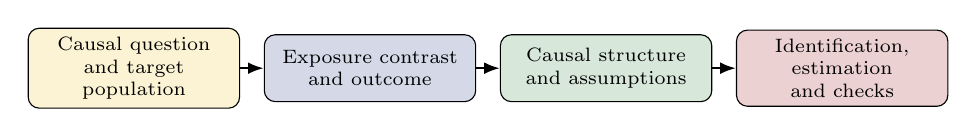
\begin{tikzpicture}[
  node distance=0.30cm,
  box/.style={draw, rounded corners, align=center, minimum height=0.85cm,
              text width=2.45cm, font=\scriptsize},
  arrow/.style={-{Latex[length=2mm]}, thick}
]
\node[box, fill=ukudlaLightYellow] (question) {Causal question\\and target population};
\node[box, fill=ukudlaLightBlue, right=of question] (contrast) {Exposure contrast\\and outcome};
\node[box, fill=ukudlaLightGreen, right=of contrast] (assumptions) {Causal structure\\and assumptions};
\node[box, fill=ukudlaLightRed, right=of assumptions] (analysis) {Identification,\\estimation and checks};
\draw[arrow] (question) -- (contrast);
\draw[arrow] (contrast) -- (assumptions);
\draw[arrow] (assumptions) -- (analysis);
\end{tikzpicture}
\end{center}

\vspace{0.35cm}

\begin{itemize}
  \item Define what intervention or exposure difference the effect represents.
  \item State which variables occur before, during and after the exposure.
  \item Use domain knowledge to identify common causes and selection processes.
  \item Decide whether the available data can identify the intended effect.
\end{itemize}

\vspace{0.25cm}

\centering
\textcolor{ukudlaRed}{Causal analysis is a research design supported by models---not a regression command.}

\end{frame}
%--------------------------------------------------



\section{Concepts}


%--------------------------------------------------
% CONTENT SLIDE 3/10
\begin{frame}{Define the estimand before the estimator}

\small

\begin{columns}[T]

\column{0.31\textwidth}

\textbf{Target quantity}

\begin{itemize}
  \item target population;
  \item exposure and contrast;
  \item outcome and time horizon; and
  \item aggregation level.
\end{itemize}

\column{0.31\textwidth}

\textbf{Potential outcomes}

\begin{itemize}
  \item $Y_i(a)$: outcome under condition $a$;
  \item individual effect: $Y_i(a_1)-Y_i(a_0)$; and
  \item average effect over target units.
\end{itemize}

\column{0.33\textwidth}

\textbf{Fundamental problem}

\begin{itemize}
  \item one unit experiences one realized exposure;
  \item the alternative outcome is unobserved; and
  \item identification requires valid comparisons.
\end{itemize}

\end{columns}

\vspace{0.35cm}

\begin{beamercolorbox}[rounded=true,sep=8pt]{block body}
``Apply treatment A'' must specify its dose, timing, delivery, comparator and target unit. Otherwise the causal contrast is ambiguous.
\end{beamercolorbox}

\end{frame}
%--------------------------------------------------


%--------------------------------------------------
% CONTENT SLIDE 4/10
\begin{frame}{A causal diagram makes assumptions inspectable}

\small

\begin{columns}[T]

\column{0.54\textwidth}

\centering
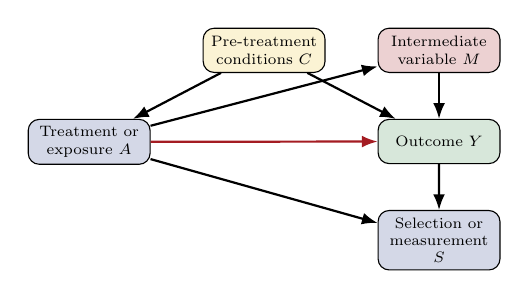
\begin{tikzpicture}[
  scale=0.78,
  transform shape,
  node distance=0.75cm and 0.85cm,
  causalnode/.style={draw, rounded corners, align=center, minimum height=0.72cm,
                   text width=1.75cm, font=\scriptsize},
  arrow/.style={-{Latex[length=2mm]}, thick}
]
\node[causalnode, fill=ukudlaLightYellow] (climate) {Pre-treatment\\conditions $C$};
\node[causalnode, fill=ukudlaLightBlue, below left=of climate] (precip) {Treatment or\\exposure $A$};
\node[causalnode, fill=ukudlaLightGreen, below right=of climate] (yield) {Outcome $Y$};
\node[causalnode, fill=ukudlaLightRed, right=of climate] (management) {Intermediate\\variable $M$};
\node[causalnode, fill=ukudlaLightBlue, below=of yield] (countrytime) {Selection or\\measurement $S$};
\draw[arrow] (climate) -- (precip);
\draw[arrow] (climate) -- (yield);
\draw[arrow, ukudlaRed] (precip) -- (yield);
\draw[arrow] (precip) -- (management);
\draw[arrow] (management) -- (yield);
\draw[arrow] (precip) -- (countrytime);
\draw[arrow] (yield) -- (countrytime);
\end{tikzpicture}

\column{0.42\textwidth}

\textbf{Use the diagram to ask}

\begin{itemize}
  \item Which variables cause both exposure and outcome?
  \item Which paths should adjustment block?
  \item Is a variable a mediator or collider?
  \item Which causes are measured adequately?
\end{itemize}

\vspace{0.20cm}

\textcolor{ukudlaRed}{Arrows encode assumptions, not correlations discovered by software.}

\end{columns}

\end{frame}
%--------------------------------------------------


%--------------------------------------------------
% CONTENT SLIDE 5/10
\begin{frame}{Regression estimates a conditional association}

\small

\begin{center}
\Large
$Y_i = \beta_0 + \beta_1 A_i + \boldsymbol{\gamma}^{\mathsf T}\mathbf{C}_i + \varepsilon_i$
\end{center}

\vspace{0.25cm}

\begin{columns}[T]

\column{0.47\textwidth}

\textbf{Model components}

\begin{itemize}
  \item $Y_i$: outcome for target unit $i$;
  \item $A_i$: treatment or exposure condition;
  \item $\mathbf{C}_i$: selected pre-exposure covariates;
  \item $\boldsymbol{\gamma}$: their conditional coefficients; and
  \item $\varepsilon_i$: unexplained model deviation.
\end{itemize}

\column{0.47\textwidth}

\textbf{Coefficient interpretation}

\begin{itemize}
  \item $\beta_1$: modeled outcome contrast per exposure contrast;
  \item conditional on included pre-exposure covariates;
  \item linear and constant unless the model says otherwise;
  \item causal only when identification assumptions hold.
\end{itemize}

\end{columns}

\vspace{0.20cm}

\centering
\textcolor{ukudlaRed}{Adding controls changes the comparison; it does not automatically remove bias.}

\end{frame}
%--------------------------------------------------


%--------------------------------------------------
% CONTENT SLIDE 6/10
\begin{frame}{Identification requires assumptions beyond regression}

\small

\begin{tabularx}{\textwidth}{@{}p{0.23\textwidth}X X@{}}
\toprule
\textbf{Assumption} & \textbf{Meaning} & \textbf{Questions across study designs} \\
\midrule
Consistency & Observed outcome matches the specified exposure condition & Are protocol, dose and timing well defined? \\
Exchangeability & Treatment groups are comparable conditional on design or covariates & Was treatment randomized; were common causes measured? \\
Positivity & Relevant contrasts occur for all adjustment profiles & Does every block, site or subgroup support the contrast? \\
No interference & One unit's treatment does not change another unit's outcome & Can plots, samples, farms or regions affect each other? \\
Measurement & Exposure, outcome and confounders represent intended concepts & Are instruments, assays and reported variables valid? \\
\bottomrule
\end{tabularx}

\vspace{0.15cm}

\begin{beamercolorbox}[rounded=true,sep=6pt]{block body}
Identification connects the causal estimand to the observed-data distribution. If essential assumptions are implausible, a precise estimate can remain causally uninterpretable.
\end{beamercolorbox}

\end{frame}
%--------------------------------------------------


%--------------------------------------------------
\section{Application}
% CONTENT SLIDE 7/10

\begin{frame}{Diagnostics assess the model, not the causal design}

\small

\begin{columns}[T]

\column{0.47\textwidth}

\textbf{Model checks can reveal}

\begin{itemize}
  \item nonlinear exposure-outcome patterns;
  \item changing residual variance;
  \item influential observations;
  \item batch, block, site, temporal or grouped residual structure; and
  \item sensitivity to transformations and specification.
\end{itemize}

\column{0.47\textwidth}

\textbf{They cannot establish}

\begin{itemize}
  \item absence of unmeasured confounding;
  \item a well-defined intervention;
  \item correct causal direction;
  \item adequate measurement; or
  \item transferability beyond the target data.
\end{itemize}

\end{columns}

\vspace{0.35cm}

\begin{beamercolorbox}[rounded=true,sep=8pt]{block body}
Confidence intervals quantify sampling uncertainty under the model. They do not include unknown confounding, measurement error or misspecified causal structure.
\end{beamercolorbox}

\end{frame}
%--------------------------------------------------



%--------------------------------------------------
% CONTENT SLIDE 8/10
\begin{frame}{Specify a causal analysis before estimation}

\small

\begin{columns}[T]

\column{0.47\textwidth}

\textbf{Provisional target}

\begin{itemize}
  \item units and target population;
  \item a well-defined exposure or intervention;
  \item outcome and timing;
  \item a meaningful exposure contrast; and
  \item target period and setting.
\end{itemize}

\column{0.47\textwidth}

\textbf{Required design work}

\begin{itemize}
  \item draw and justify a causal diagram;
  \item distinguish pre-exposure confounders from mediators;
  \item evaluate assignment or overlap within relevant groups;
  \item document unmeasured causes and exposure ambiguity; and
  \item decide whether the effect is identifiable.
\end{itemize}

\end{columns}

\vspace{0.25cm}

\centering
\textcolor{ukudlaRed}{Observed exposure variation is not automatically equivalent to a controlled intervention.}

\end{frame}
%--------------------------------------------------


%--------------------------------------------------
% CONTENT SLIDE 9/10
\begin{frame}{Compare estimates---then challenge their interpretation}

\small

\begin{center}
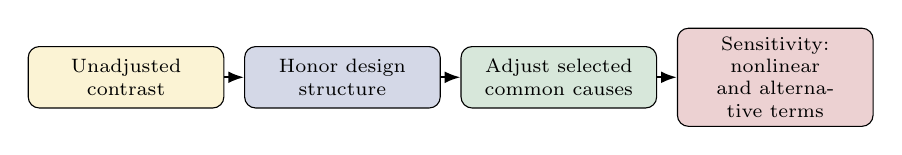
\begin{tikzpicture}[
  node distance=0.25cm,
  box/.style={draw, rounded corners, align=center, minimum height=0.78cm,
              text width=2.25cm, font=\scriptsize},
  arrow/.style={-{Latex[length=2mm]}, thick}
]
\node[box, fill=ukudlaLightYellow] (m1) {Unadjusted\\contrast};
\node[box, fill=ukudlaLightBlue, right=of m1] (m2) {Honor design\\structure};
\node[box, fill=ukudlaLightGreen, right=of m2] (m3) {Adjust selected\\common causes};
\node[box, fill=ukudlaLightRed, right=of m3] (m4) {Sensitivity: nonlinear\\and alternative terms};
\draw[arrow] (m1) -- (m2);
\draw[arrow] (m2) -- (m3);
\draw[arrow] (m3) -- (m4);
\end{tikzpicture}
\end{center}

\vspace{0.25cm}

\begin{itemize}
  \item Report the target coefficient or contrast, uncertainty and effective $n$.
  \item Explain how the comparison changes across specifications.
  \item Inspect exposure overlap, residual plots, influence and temporal structure.
  \item Separate statistical precision from identification credibility.
  \item Label estimates as adjusted associations when causal assumptions remain unsupported.
\end{itemize}

\vspace{0.15cm}

\centering
\textcolor{ukudlaRed}{Specification sensitivity is evidence to interpret---not a contest to find significance.}

\end{frame}
%--------------------------------------------------


%--------------------------------------------------
\section{Key Message}
% CONTENT SLIDE 10/10

\begin{frame}{Key message: causal meaning comes from design}

\small

\begin{columns}[T]

\column{0.47\textwidth}

\textbf{Reproducible artifacts}

\begin{itemize}
  \item causal question and estimand;
  \item causal diagram with justification;
  \item model specification table;
  \item coefficient and uncertainty table;
  \item diagnostics and sensitivity results; and
  \item code-linked explanatory report.
\end{itemize}

\column{0.47\textwidth}

\textbf{Conclusion must distinguish}

\begin{itemize}
  \item what the data describe;
  \item what the models estimate;
  \item which assumptions support identification;
  \item which assumptions remain doubtful; and
  \item which additional data or design are needed.
\end{itemize}

\end{columns}

\vspace{0.30cm}

\begin{beamercolorbox}[rounded=true,sep=8pt]{block body}
A credible causal analysis may conclude that the available data identify only adjusted associations. Making that boundary explicit is a scientific result, not a failure.
\end{beamercolorbox}

\vspace{0.15cm}

\centering
\textcolor{ukudlaRed}{Estimate transparently---and earn the causal interpretation through design and assumptions.}

\end{frame}
%--------------------------------------------------


%--------------------------------------------------
\begin{frame}[plain,noframenumbering]{Supported by}

  South African government and the National Research Foundation

  \begin{flushleft}
    \includegraphics[trim=0cm 0cm 0cm 0cm, clip, width=0.50\textwidth]{./logos/ukudla_south_african_sponsors.pdf}
  \end{flushleft}

  German government and the German Academic Exchange Service

  \begin{flushleft}
    \includegraphics[trim=0cm 0cm 0cm 0cm, clip, width=1.00\textwidth]{./logos/ukudla_german_sponsors.pdf}
  \end{flushleft}

\end{frame}
%--------------------------------------------------

\end{document}
